% RansKnow dataset paper -- skeleton
%
% Status as of this draft: Dataset Construction, Label-Quality Audit, and
% Interpretability/Perturbation-Robustness (Phase 5) describe work that is
% DONE and verified against the actual repository state. Baselines (Phase 1)
% are also complete but explicitly weak-label-only: this project does not
% include an independent human-annotated evaluation set (see the scope note
% at the end of Section 3 -- external annotator recruitment required
% institutional ethics approval this project doesn't have, and a
% single-investigator pass was decided against as still too close to the
% pipeline being evaluated). Every downstream number is reported as
% agreement with the audited extraction pipeline, not as verified accuracy.
% Uncertainty (Sec 5) and Conformal Prediction (Sec 6) are reframed
% accordingly -- their formal properties still hold relative to the
% weak-label distribution, just with a correspondingly weaker
% interpretation, stated explicitly rather than implied. OOD Detection
% (Sec 7) needs no such caveat: it doesn't depend on label correctness at
% all, only on whether the model's own confidence/embedding behavior
% differs on distributionally-shifted input. Remaining \todo{} markers are
% real open items, not silent gaps.
%
% Target: NeurIPS 2026 Evaluations & Datasets Track template (the 2026
% submission deadline, 2026-05-06, has already passed by the time this
% conversion was done -- targeting the 2027 cycle instead, using the 2026
% style file as the closest available reference; year-to-year formatting
% changes are typically minor. Swap in neurips_2027.sty (drop-in, same
% [eandd] option) once it's published, and update every "2026" reference
% below (this comment, \bibliographystyle notes, FundingDisclosure URL in
% the ack block) to 2027.
%
% Official files (neurips_2026.sty, checklist.tex) fetched from
% https://media.neurips.cc/Conferences/NeurIPS2026/Formatting_Instructions_For_NeurIPS_2026.zip
% -- unmodified, per submission requirements ("tweaking the style files
% may be grounds for desk rejection").

\documentclass{article}

% Track options, mirroring the official shell's own commenting convention:
%   (submission/default, current)   \usepackage[eandd]{neurips_2026}
%   (arXiv/preprint)                \usepackage[eandd, preprint]{neurips_2026}
%   (camera-ready, post-acceptance) \usepackage[eandd, final]{neurips_2026}
% Default (no track option, no final/preprint) auto-anonymizes the
% \author block below to "Anonymous Author(s)" -- do NOT hand-edit author
% info for submission; the class handles it.
\usepackage[eandd]{neurips_2026}

\usepackage[utf8]{inputenc}
\usepackage[T1]{fontenc}
\usepackage{hyperref}
\usepackage{url}
\usepackage{booktabs}
\usepackage{amsfonts}
\usepackage{nicefrac}
\usepackage{microtype}
\usepackage{xcolor}
\usepackage{graphicx}
\usepackage{amsmath}
\usepackage{amssymb}
\usepackage{algorithm}
\usepackage{algpseudocode}
\usepackage[capitalize]{cleveref}
% Do NOT load geometry separately -- neurips_2026.sty sets margins itself
% via \newgeometry{...}; loading it again risks exactly the "tweaking the
% style files" desk-rejection warning in the submission instructions.

\hypersetup{colorlinks=true, linkcolor=blue, citecolor=blue, urlcolor=blue}

% Deliberately not using the todonotes package: its margin-note/inline
% float mechanism collided with this document's real tables and produced
% an unrecoverable "Float(s) lost" error (confirmed by isolating with
% [disable] -- the document compiles cleanly without it). This does the
% same job -- visually flag incomplete sections -- as plain paragraph
% text, which can't collide with anything. The optional [inline] argument
% below is accepted and ignored, so every existing \todo[inline]{...} /
% \todo{...} call site works unchanged.
\newcommand{\todo}[2][]{\par\medskip\noindent\textcolor{red}{\textbf{[TODO]}}\ #2\par\medskip}

\title{RansKnow: An Open Dataset of Ransomware-Related YouTube\\
Transcripts with MITRE ATT\&CK Annotations}

\author{
  Henry Kabuye \\
  \texttt{[affiliation -- TODO before submission]} \\
  \texttt{kabuyehenry2017@gmail.com}
}

\date{}

\begin{document}
\maketitle

\begin{abstract}
\todo[inline]{Draft, not final. Should state: (1) what RansKnow is
(1{,}128 video records, 1{,}034 transcripts, 92 cybersecurity YouTube
channels, MITRE ATT\&CK-aligned regex features); (2) the paper's actual
contribution is arguably the label-quality audit methodology as much as
the corpus itself -- Section~\ref{sec:audit} found that a naive
keyword-matched family label collided with ordinary English words
(\texttt{play}, \texttt{hive}, \texttt{cactus}, \dots) badly enough to
inflate the single most-detected ransomware family by $\sim$3.5$\times$,
and Section~\ref{sec:interpretability}'s counterfactual analysis shows a
trained classifier partially inherited that same word-level fragility
even after the fix; (3) state plainly, in the abstract itself, not just
in a limitations section: baseline results (Section~\ref{sec:baselines})
are weak-label agreement scores, not independently verified accuracy --
this project does not include human-annotated ground truth (see the
scope note in Section~\ref{sec:gold-scope}); (4) headline OOD-robustness
numbers, which don't depend on that caveat.}
\end{abstract}

\section{Introduction}
\label{sec:intro}

\todo[inline]{The gap: no open, transcript-level ransomware knowledge
corpus with MITRE ATT\&CK-aligned annotations. Motivate why YouTube
security content specifically (volume, diversity of source -- vendor
threat-intel channels, DFIR conferences, independent researchers -- versus
e.g. only vendor blog posts). State the paper's contributions as a list:
(1) the corpus; (2) the label-quality audit methodology and its concrete
findings (Section~\ref{sec:audit}); (3) the experiment framework and
weak-label baseline results (Section~\ref{sec:baselines}), reported as
agreement with the audited extraction pipeline -- state directly here,
not just in Limitations, that no independent human-annotated ground
truth was collected for this project (Section~\ref{sec:gold-scope}); (4)
out-of-distribution robustness results (Section~\ref{sec:ood}), which are
not subject to that caveat; (5) counterfactual and perturbation-robustness
interpretability results (Section~\ref{sec:interpretability}).}

\section{Related Work}
\label{sec:related}

\todo[inline]{Three threads: (a) existing ransomware/threat-intel datasets
(structured IOC feeds, MITRE ATT\&CK mapping efforts, prior ransomware
incident corpora -- note what's specific to RansKnow: raw natural-language
transcripts rather than structured feeds); (b) weak/distant supervision in
security NLP (keyword/regex-based labeling, its known failure modes); (c)
conformal prediction and OOD detection in NLP, as background for
Sections~\ref{sec:conformal} and~\ref{sec:ood} once written.}

\section{Dataset Construction}
\label{sec:construction}

RansKnow \citep{ransknow_kaggle} consists of 1{,}128 video records sourced
from 92 cybersecurity YouTube channels, of which 1{,}034 have an extracted
transcript with real content; the remaining 94\footnote{\todo{Verify this figure against the
    live dataset before submission -- $1128 - 1034 = 94$, but confirm this
    is failed transcript extraction and not something else, e.g. videos
    excluded post-fetch.}} could not be transcribed by any method in the
fetch cascade.

\subsection{Channel selection}
Channels were curated in two batches. Batch 1 (50 channels, \texttt{C01}--\texttt{C50})
covers established DFIR vendors, security conferences, and independent
researchers. Batch 2 (51 candidate channels, \texttt{C51}--\texttt{C101})
expanded coverage into threat-intelligence vendors, additional conferences,
and OT/ICS-security and government channels; 42 of the 51 candidates
yielded usable transcripts, 1 was a confirmed duplicate of an existing
Batch 1 channel, 4 had no discoverable dedicated YouTube channel, and 4
resolved to real channels with zero ransomware-keyword-matching content in
their upload history. \todo{Cite the specific channel registry files
    (\texttt{rubrics/Dataset\_Channel\_Registry\_*.xlsx}) and consider a
    full channel table as a supplementary table rather than inline.}

\subsection{Video selection}
Within each channel, videos were selected by scanning recent uploads for a
fixed keyword list (\texttt{ransomware}, \texttt{extortion},
\texttt{lockbit}, \texttt{incident response}, \dots; full list in
Appendix~\ref{app:keywords}) matched against title and description, capped
at 20 videos per channel and a minimum duration of 5 minutes. \todo{Report
    the actual keyword list and discuss selection bias explicitly: this
    is a convenience sample conditioned on channel operators' own titling
    and description-writing behavior, not a random sample of ransomware
    discourse.}

\subsection{Transcript acquisition}
\label{sec:transcripts}
Transcripts were acquired via a three-stage cascade: (1) the YouTube Data
API's official captions where available; (2) \texttt{yt-dlp}'s
auto-generated captions; (3) local Whisper transcription as a fallback.
\textbf{This cascade matters more than a footnote}: only 74 of 1{,}034
transcripts (7.2\%) came from official captions. 959 (92.7\%) are ASR
output -- 554 from \texttt{whisper\_base} (the smallest, least accurate
Whisper checkpoint) and 405 from a local Whisper fallback, 1 from
\texttt{yt-dlp} captions. \todo{This is Finding B from the label-quality
    audit (Section~\ref{sec:audit}). Decide whether to present it once,
    here, or duplicate the framing in both sections -- probably present the
    raw fact here and the downstream implication (jargon
    mistranscription risk) in Section~\ref{sec:audit}.}

\section{Label-Quality Audit}
\label{sec:audit}

The Knowledge Agent pipeline (\texttt{Scripts/knowledge\_agent.py})
extracts structured features from every transcript via regex matching:
ransomware family mentions (against a maintained alias list), MITRE
ATT\&CK tactic mention counts across 10 tactics, offensive tool mentions
across 8 tools, and platform signals (Windows/Linux/ESXi). Three concrete
problems were found and are described here rather than left as an implicit
caveat, because a downstream classifier trained on these labels inherits
whatever bias they contain.

\subsection{Finding A: generic-word alias collisions}
\label{sec:finding-a}
Nine of 41 family aliases collide with common English or business words
(\texttt{play}, \texttt{hive}, \texttt{cactus}, \texttt{agenda},
\texttt{clop}, \texttt{inc}, \texttt{maze}, \texttt{medusa},
\texttt{royal}) -- identified programmatically via dictionary lookup
against \texttt{/usr/share/dict/words}, then confirmed by manual
transcript inspection (e.g. \texttt{hive} matching ``registry hive,'' a
routine DFIR term, rather than Hive ransomware). A windowed-context
disambiguation fix (requiring a ransomware-context term within
$\sim$15 tokens of the match) was applied and reduces false-positive
volume substantially without eliminating it -- residual false positives
still occur when context vocabulary is itself dense (see
\texttt{Scripts/audit\_family\_aliases.py} for the audit methodology and
\Cref{tab:alias-audit} for before/after counts).

\begin{table}[htbp]
\centering
\caption{Before/after family mention counts for the 9 flagged aliases,
  windowed-context disambiguation applied. \texttt{Play} alone accounted
  for 386 of 494 (78\%) of all family-tagged videos before the fix.}
\label{tab:alias-audit}
\begin{tabular}{lrrr}
\toprule
Family & Before & After & Dropped \\
\midrule
Play    & 386 & 111 & 275 \\
Qilin   &  88 &  21 &  67 \\
Hive    &  23 &  10 &  13 \\
Maze    &  11 &   5 &   6 \\
Royal   &  28 &  19 &   9 \\
INC     &  10 &   7 &   3 \\
Cactus  &   9 &   6 &   3 \\
Cl0p    &  11 &  11 &   0 \\
Medusa  &   7 &   7 &   0 \\
\bottomrule
\end{tabular}
\end{table}

\subsection{Finding B: ASR-dominated transcript quality}
As noted in Section~\ref{sec:transcripts}, 92.7\% of transcripts are ASR
output rather than official captions. \todo{Run the Phase 0.4 spot-check
    (manual comparison of ASR output against source audio for a fixed
    jargon term list -- \texttt{LockBit}, \texttt{Mimikatz},
    \texttt{PsExec}, \texttt{Cobalt Strike}, \texttt{rclone},
    \texttt{BloodHound} -- across the whisper-transcribed subset) and
    report a measured word-error-rate-on-jargon figure here. Aggregate
    detection-rate comparisons across \texttt{Transcript\_Provider} did
    not show an obvious gap, which is not the same as no effect --
    individual mistranscriptions of rare jargon can matter without moving
    an aggregate rate.}

\subsection{Scope: no independent ground truth}
\label{sec:gold-scope}
An earlier design stage of this project planned a held-out, independently
annotated evaluation subset (180 videos, stratified by channel type,
year, and current family-count) specifically to break the circularity of
evaluating a classifier against the same weak-label pipeline it was
trained on. That subset was never annotated. External annotator
recruitment required institutional ethics approval not available to this
project; a single-investigator pass was considered as a fallback and
rejected as still too close to the system under evaluation to serve as
independent ground truth in a way worth claiming in a paper.

The consequence is stated here plainly, and repeated at the point every
affected result is reported, rather than left as a single Limitations
bullet a reader could miss: \textbf{every quantitative result in
Section~\ref{sec:baselines} onward, with the explicit exception of
Section~\ref{sec:ood}'s out-of-distribution results, measures agreement
with the audited Knowledge Agent extraction pipeline (Section~\ref{sec:audit}),
not verified accuracy against human judgment.} Section~\ref{sec:audit}
demonstrates concretely that this pipeline's labels contain real,
non-trivial error even after the disambiguation fix (Finding A); nothing
downstream corrects for that. Readers should treat macro-F1 and
calibration numbers in this paper as characterizing how well models
reproduce a specific, imperfect, documented extraction process --
not as claims about ransomware-domain understanding in an absolute
sense. Section~\ref{sec:limitations} returns to this as the paper's
central limitation.

\section{Task Definitions and Baselines}
\label{sec:baselines}

Five prediction tasks are defined over the corpus: ransomware family
(multi-label, 18 classes after excluding 3 singleton-occurrence classes,
see \Cref{tab:tasks}), dominant MITRE tactic (multi-class, 11 classes),
platform signal (multi-class, 4 classes), offensive tool mentions
(multi-label, 7 classes after excluding \texttt{MegaNZ}, which has zero
occurrences in the corpus), and a ransomware-relevance binary screen
(derived, not a stored column: \texttt{Family\_Count > 0 OR
  Tactic\_Impact > 0}).

\begin{table}[htbp]
\centering
\caption{Task taxonomy.}
\label{tab:tasks}
\begin{tabular}{llrl}
\toprule
Task & Type & Classes & Label source \\
\midrule
Family              & multi-label            & 18 & alias regex match (audited, \S\ref{sec:finding-a}) \\
Dominant tactic      & multi-class (+none)    & 11 & max of 10 tactic-pattern counts \\
Platform signal      & multi-class (+none)    &  4 & max of 3 platform-pattern counts \\
Tool mentions        & multi-label            &  7 & per-tool regex match \\
Ransomware-relevant   & binary                 &  2 & derived \\
\bottomrule
\end{tabular}
\end{table}

\subsection{Model ladder and validation protocol}
Each task is evaluated over three feature representations (structured
Knowledge Agent columns, TF-IDF, mean-pooled sentence embeddings\footnote{384-dim
  \texttt{all-MiniLM-L6-v2}, chunked at $\sim$200 words per chunk and
  mean-pooled, computed via a dedicated Python environment
  (\texttt{torch}~2.5.1) since the reference implementation's default
  environment ships an older \texttt{torch} that cannot satisfy
  \texttt{sentence\_transformers}' requirements; see
  \texttt{Scripts/precompute\_embeddings.py}.}) and five models (the
rule-based Knowledge Agent itself as baseline 0, Logistic Regression,
Linear SVM, Random Forest, LightGBM), under three cross-validation
protocols: stratified random $k$-fold, \texttt{GroupKFold} by
\texttt{Channel\_ID} (to detect channel-style leakage -- a model can learn
``this is CrowdStrike's narration style'' instead of the content), and a
temporal split (train pre-2024, test 2024+, since 79\% of the corpus is
from 2024 onward).

\subsection{Results}
\label{sec:baseline-results}
Per Section~\ref{sec:gold-scope}, every number in this section is
weak-label agreement -- how well a model reproduces the Knowledge
Agent's own extraction, not verified accuracy. The rule-based Knowledge
Agent baseline scores a tautological macro-F1 of 1.000 on every task
(checked against its own labels by construction; included as baseline 0,
not as evidence of anything) and is omitted from \Cref{tab:results}
accordingly.

\begin{table}[htbp]
\centering
\caption{Best stratified-CV macro-F1 per task, across every representation
  (structured / TF-IDF / embedding) and trained model (LogReg, Linear SVM,
  Random Forest, GBM) tried. Weak-label agreement, not verified accuracy
  (\S\ref{sec:gold-scope}).}
\label{tab:results}
\begin{tabular}{lllr}
\toprule
Task & Best representation & Best model & Macro-F1 \\
\midrule
Ransomware-relevant & TF-IDF     & GBM    & 0.903 \\
Dominant tactic      & structured & GBM    & 0.813 \\
Platform signal       & TF-IDF     & GBM    & 0.606 \\
Tool mentions         & TF-IDF     & LogReg & 0.200 \\
Family                 & embedding  & LogReg & 0.129 \\
\bottomrule
\end{tabular}
\end{table}

Two patterns worth naming, both consistent with Section~\ref{sec:interpretability}'s
independent checks: (1) tree models (GBM in particular) are the strongest
model wherever tested, and structured features remain the strongest
representation specifically for \texttt{dominant\_tactic} -- unsurprising,
since those features are numerically close to the counts the label itself
was derived from; (2) \texttt{family} and \texttt{tool} are weak under
every representation and model combination tried (family never exceeds
0.13 macro-F1; tool is additionally unstable across CV splits, ranging
0.03--0.20). This is not obviously a framework or tuning limitation --
Section~\ref{sec:interpretability}'s length and channel-identity confound
checks rule out two of the more common alternative explanations for weak
tabular/text-classification performance, leaving weak-label ceiling
(\S\ref{sec:gold-scope}) and genuine class sparsity (Section~\ref{sec:baselines}'s
18-class family / 7-class tool taxonomies, several classes with single-digit
support) as the remaining candidate explanations. \todo{Full
    task$\times$representation$\times$model$\times$split table as
    supplementary material, or as a figure once uncommented below; cite
    \texttt{outputs/experiments/phase1\_*.csv} directly.}

% \begin{figure}[htbp]
%   \centering
%   \includegraphics[width=0.9\textwidth]{figures/fig_baselines_macro_f1.pdf}
%   \caption{Macro-F1 by task, model, and CV protocol (weak-label agreement,
%     \S\ref{sec:gold-scope}).}
%   \label{fig:baselines}
% \end{figure}

\section{Uncertainty Quantification}
\label{sec:uncertainty}
\textbf{Scope note (\S\ref{sec:gold-scope} applies here directly):}
calibration is normally reported against ground truth -- does an 80\%-confidence
prediction turn out correct roughly 80\% of the time. Without independent
labels, the only calibration target available here is the weak-label
distribution itself, which changes what a well-calibrated result would
mean: a model perfectly calibrated against its own training signal has
learned to be a confident, well-calibrated echo of a regex, not
necessarily a well-calibrated model of ransomware content. This section
is retained, with that meaning made explicit at every reported number,
because reliability diagrams and Expected Calibration Error against the
weak labels are still informative about a narrower question worth
answering: does a model's confidence track its \emph{agreement with the
extraction pipeline}, or is it uniformly overconfident regardless of
agreement. The latter would be a red flag on its own.

\subsection{Calibration against weak labels}
\label{sec:uncertainty-calibration}
For a multiclass task, let $\hat p(\cdot \mid x)$ be the trained model's
predicted class distribution for input $x$, and let $\hat c(x) =
\arg\max_c \hat p(c\mid x)$ with confidence $\hat p_{\max}(x) =
\max_c \hat p(c\mid x)$. Agreement with the weak label $y^{\mathrm{KA}}(x)$
(the Knowledge Agent's own extraction) is $a(x) = \mathbb{1}[\hat c(x) =
y^{\mathrm{KA}}(x)]$. For the two multi-label tasks (\texttt{family},
\texttt{tool}), whose models are independent per-class binary
classifiers (\Cref{sec:baselines}), each (sample, class) pair
$(x,k)$ is treated as its own calibration point, with confidence
$\hat p_{\max}(x,k) = \max\bigl(\hat p_k(x), 1-\hat p_k(x)\bigr)$ and
agreement against the binary weak label thresholded at $0.5$.

Reliability is summarized with $B{=}10$ equal-width confidence bins
$\{I_b\}_{b=1}^{B}$ and the standard Expected Calibration Error,
\begin{equation}
\label{eq:ece}
\mathrm{ECE} \;=\; \sum_{b=1}^{B} \frac{|S_b|}{N}
  \left\lvert \operatorname{acc}(S_b) - \operatorname{conf}(S_b) \right\rvert,
\qquad
S_b = \{x : \hat p_{\max}(x) \in I_b\},
\end{equation}
where $\operatorname{acc}(S_b) = \frac{1}{|S_b|}\sum_{x \in S_b} a(x)$ and
$\operatorname{conf}(S_b) = \frac{1}{|S_b|}\sum_{x \in S_b} \hat p_{\max}(x)$.
Per the scope note above, $a(x)$ measures agreement with $y^{\mathrm{KA}}$,
not correctness, so \cref{eq:ece} is a \emph{weak-label ECE}. The
headline number below the scope note is the confident-disagreement
rate at threshold $\tau=0.9$,
\begin{equation}
\label{eq:cdr}
\mathrm{CDR}_\tau \;=\; \frac{1}{N}\sum_{i=1}^N
  \mathbb{1}\!\left[\hat p_{\max}(x_i) > \tau\right]\cdot\bigl(1-a(x_i)\bigr),
\end{equation}
the closest available analogue to a ``confidently wrong'' rate without
independently verified labels to actually be wrong against.

Each task is evaluated on the 5-fold stratified out-of-fold predictions
of its best (feature, model) combination from \Cref{tab:results}, except
\texttt{family}, whose best combination (embedding representation) needs
the dedicated environment described in \Cref{sec:baselines}'s footnote
and is reported without a calibration curve here.

\begin{table}[htbp]
\centering
\caption{Weak-label calibration (\Cref{eq:ece,eq:cdr}) and the RF
  tree-vote entropy proxy (\Cref{eq:entropy}), best (feature, model) per
  task. $N$ is the number of (sample) or (sample, class) calibration
  points. Entropy AUROC is how well entropy alone separates agreement
  from disagreement with the weak label (\Cref{alg:rf-entropy}).}
\label{tab:calibration}
\begin{tabular}{lrrrrr}
\toprule
Task & $N$ & ECE & $\mathrm{CDR}_{0.9}$ & Entropy (agree/disagree) & Entropy AUROC \\
\midrule
Relevance        & 1034 & 0.079 & 0.071 & 0.910 / 0.980 & 0.769 \\
Dominant tactic   & 1034 & 0.051 & 0.043 & 0.275 / 0.551 & 0.860 \\
Platform          & 1034 & 0.110 & 0.104 & 0.717 / 0.769 & 0.675 \\
Tool (per-label)  & 7238 & 0.016 & 0.016 & 0.121 / 0.271 & 0.977 \\
Family (per-label)& 1034 & --    & --    & 0.095 / --     & --    \\
\bottomrule
\end{tabular}
\end{table}

\Cref{fig:reliability} plots the reliability curves underlying
\Cref{tab:calibration}. Two things worth naming honestly rather than
smoothing over: first, per-bin counts are small (single digits to low
tens per bin at $N{=}1034$), so individual bin heights are noisy --
the curves are directionally informative, not point-estimate-precise.
Second, \texttt{family}'s row has no ECE/CDR: its calibration point is
unavailable in this environment (as above), so only the RF tree-vote
entropy proxy, computed on the TF-IDF fallback representation, is
reported for it, and even that proxy has no ``disagree'' entries to
average -- at the per-(sample, class) level, most of \texttt{family}'s
18 classes are negative for most samples, so the majority-class
prediction (``absent'') agrees with the weak label on essentially every
RF-on-TF-IDF calibration point despite the task's low macro-F1 in
\Cref{tab:results}, which weights all 18 classes equally rather than by
prevalence. Both readings are correct simultaneously; they are just
answering different questions (per-pair agreement vs.\ per-class
balanced performance).

\begin{figure}[htbp]
  \centering
  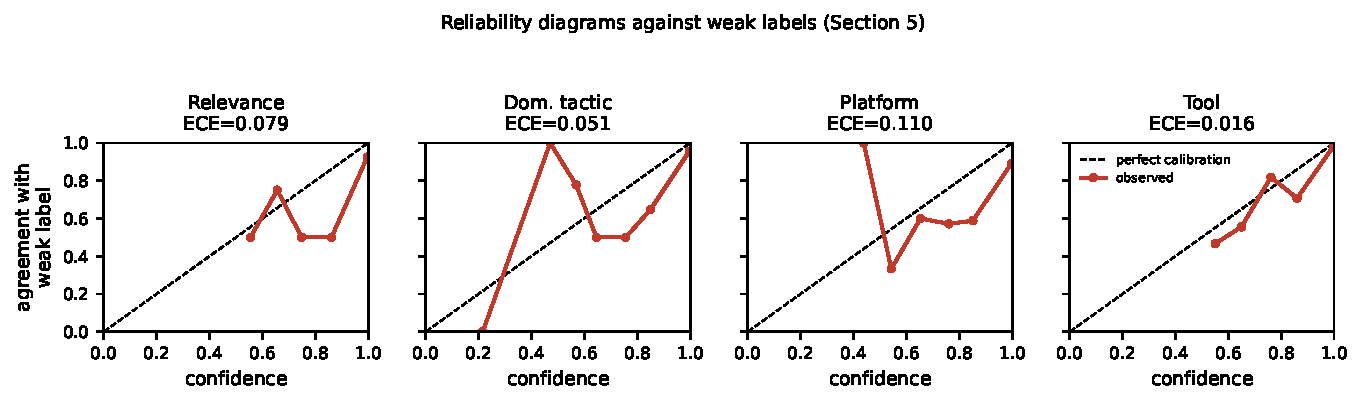
\includegraphics[width=\textwidth]{figures/fig_uncertainty_reliability.pdf}
  \caption{Reliability diagrams against weak labels, one panel per task
    with a usable calibration curve (\Cref{tab:calibration}). Diagonal
    is perfect calibration.}
  \label{fig:reliability}
\end{figure}

\subsection{A free uncertainty proxy: Random Forest tree-vote entropy}
\label{sec:uncertainty-rf}
Reliability diagrams need a held-out calibration protocol; a Random
Forest offers a per-prediction uncertainty signal with no separate
calibration step. For an input $x$ and a forest of $T$ trees producing
individual (hard) predictions $t_1(x),\dots,t_T(x)$ over $K$ classes, let
$\pi_c(x) = \frac{1}{T}\sum_{j=1}^T \mathbb{1}[t_j(x)=c]$ be the empirical
vote share for class $c$. The normalized tree-vote entropy is
\begin{equation}
\label{eq:entropy}
H(x) \;=\; -\frac{1}{\log K}\sum_{c=1}^{K} \pi_c(x)\,\log \pi_c(x)
  \;\in\; [0,1],
\end{equation}
with $H(x){=}0$ when every tree agrees and $H(x){=}1$ at a uniform split
across all $K$ classes. For the multi-label tasks, $K{=}2$ per class and
$H(x,k)$ is averaged over classes $k$ for a per-sample summary.
\Cref{alg:rf-entropy} is the exact out-of-fold procedure used to produce
\Cref{tab:calibration}'s entropy columns.

\begin{algorithm}[htbp]
\caption{RF tree-vote entropy, 5-fold out-of-fold}
\label{alg:rf-entropy}
\begin{algorithmic}[1]
\Require dataset $\mathcal{D}$, task with label function $y(\cdot)$, feature builder $\phi$
\State $\mathcal{F} \gets$ 5 stratified folds of $\mathcal{D}$
\For{fold $(\mathcal{D}_{\mathrm{train}}, \mathcal{D}_{\mathrm{test}}) \in \mathcal{F}$}
  \State fit $\phi$ on $\mathcal{D}_{\mathrm{train}}$; fit Random Forest $\{t_j\}_{j=1}^T$ on $\phi(\mathcal{D}_{\mathrm{train}})$
  \For{$x \in \mathcal{D}_{\mathrm{test}}$}
    \State $t_j(x) \gets$ individual tree prediction, $j=1,\dots,T$ \Comment{sklearn returns internal integer-encoded classes here, not the original label strings -- see note below}
    \State recover original class labels via the fitted forest's class index before comparing to $y(x)$
    \State compute $H(x)$ via \Cref{eq:entropy}; record $a(x) = \mathbb{1}[\text{forest majority vote} = y(x)]$
  \EndFor
\EndFor
\State \Return $\{(H(x), a(x))\}_{x \in \mathcal{D}}$, pooled across folds
\end{algorithmic}
\end{algorithm}

The in-line comment in \Cref{alg:rf-entropy} records a real implementation
pitfall, not a hypothetical one: scikit-learn fits each tree in a
\texttt{RandomForestClassifier} on internally label-encoded integer
targets, so \texttt{tree.predict()} returns class \emph{indices}, not the
original label strings the ensemble's own \texttt{.predict()} returns.
Comparing tree-level votes directly against string labels without
mapping back through the fitted forest's class index silently produces
0\% apparent agreement on every multiclass task -- caught in this
project's own Phase~2 run (initial numbers showed exactly that pattern
across all three multiclass tasks simultaneously, which is what made it
legible as a bug rather than a real result) and is recorded here as a
concrete instance of the caution \Cref{sec:limitations} urges about
verifying rather than assuming standard library internals.
\Cref{tab:calibration}'s entropy AUROC column shows the proxy works well
once fixed: $0.68$--$0.98$ across tasks, best on \texttt{tool} (many
easy true negatives) and weakest on \texttt{platform}.

\section{Conformal Prediction}
\label{sec:conformal}
\textbf{Scope note:} split conformal prediction's distribution-free
coverage guarantee is a statement about exchangeability with the
calibration set, not about label correctness -- it holds formally even
when calibrated against weak labels, because the guarantee is
``the true \emph{weak} label falls in the predicted set $(1-\alpha)$ of
the time,'' not ``the true \emph{real-world} label does.'' That
distinction is the entire content of this scope note: conformal coverage
against the Knowledge Agent's labels is a well-defined, honestly
reportable number, but it validates agreement with the extraction
pipeline, not correctness. Reported as such.

\subsection{Method: split conformal with the LAC score}
\label{sec:conformal-method}
Split conformal prediction (\citealp{vovk2005algorithmic, lei2018distribution};
see \citealp{angelopoulos2023gentle} for a tutorial treatment) uses a
nonconformity score $s(x,y)$ that is small when $y$ is a plausible label
for $x$. This paper uses the least-ambiguous-set (LAC) score,
\begin{equation}
\label{eq:lac}
s(x,y) \;=\; 1 - \hat p(y \mid x),
\end{equation}
calibrated on a held-out split $\mathcal{D}_{\mathrm{calib}}$ of size $n$
disjoint from both the training and test data. The calibration threshold
uses the standard finite-sample correction,
\begin{equation}
\label{eq:qhat}
\hat q \;=\; \operatorname{Quantile}\!\left(
  \left\{s(x_i,y_i)\right\}_{i=1}^{n} ;\;
  \frac{\lceil (n+1)(1-\alpha)\rceil}{n}\right),
\end{equation}
and the prediction set for a new input $x$ is
\begin{equation}
\label{eq:predset}
C(x) \;=\; \bigl\{\, y \;:\; \hat p(y\mid x) \geq 1-\hat q \,\bigr\}.
\end{equation}
Under exchangeability of $\mathcal{D}_{\mathrm{calib}}$ and the test
point, this construction guarantees
\begin{equation}
\label{eq:coverage}
\mathbb{P}\!\left[\, y_{\mathrm{test}} \in C(x_{\mathrm{test}}) \,\right]
  \;\geq\; 1-\alpha,
\end{equation}
with $\alpha{=}0.10$ (90\% target coverage) throughout. As the scope
note above states, $y_{\mathrm{test}}$ here is the weak label
$y^{\mathrm{KA}}$: \Cref{eq:coverage} is a real, distribution-free
guarantee about agreement with the extraction pipeline, not about
real-world correctness. For \texttt{dominant\_tactic} and
\texttt{platform}, \Cref{eq:lac,eq:qhat,eq:predset} apply directly over
the task's full class vocabulary. \texttt{family} and \texttt{tool} have
no single multiclass structure to conformalize -- each is an independent
per-class binary classifier (\Cref{sec:baselines}) -- so each class $k$
gets its own binary LAC calibration and its own $\hat q_k$, and a
sample's per-label prediction sets are reported both individually and
jointly (all labels simultaneously covered).

\Cref{alg:conformal} is run for $5$ repeated random $60/20/20$
train/calibration/test splits per task, results averaged across repeats
rather than reported from one arbitrary split -- a single 20\%
calibration set at this sample size ($n{\approx}200$) is not a reliable
enough estimate of $\hat q$ to report alone.

\begin{algorithm}[htbp]
\caption{Split conformal calibration and coverage evaluation}
\label{alg:conformal}
\begin{algorithmic}[1]
\Require dataset $\mathcal{D}$, task, target coverage $1-\alpha$, repeats $R$
\For{$r = 1,\dots,R$}
  \State split $\mathcal{D}$ into $\mathcal{D}_{\mathrm{train}}$ (60\%), $\mathcal{D}_{\mathrm{calib}}$ (20\%), $\mathcal{D}_{\mathrm{test}}$ (20\%), stratified
  \State fit model on $\mathcal{D}_{\mathrm{train}}$
  \State compute $\hat q$ on $\mathcal{D}_{\mathrm{calib}}$ via \Cref{eq:lac,eq:qhat}
  \For{$x \in \mathcal{D}_{\mathrm{test}}$}
    \State build $C(x)$ via \Cref{eq:predset}; record $\mathbb{1}[y^{\mathrm{KA}}(x) \in C(x)]$ and $|C(x)|$
  \EndFor
\EndFor
\State pool test-set coverage indicators across all $R$ repeats
\State report marginal coverage, and coverage restricted to the Year${\geq}2026$ and Conference-channel slices
\end{algorithmic}
\end{algorithm}

\subsection{Results}
\label{sec:conformal-results}
\begin{table}[htbp]
\centering
\caption{Split-conformal coverage at 90\% target ($\alpha{=}0.10$), pooled
  over 5 repeats, $n{\approx}1035$ pooled test predictions per task.
  \texttt{family}/\texttt{tool} report mean per-label coverage and the
  stricter all-labels-jointly-covered rate. Set size is out of the
  task's class count ($K$) for \texttt{dominant\_tactic}/\texttt{platform},
  or out of 2 (per label) for \texttt{family}/\texttt{tool}.}
\label{tab:conformal}
\begin{tabular}{lrrrrr}
\toprule
Task & $K$ & Coverage (marginal) & Avg.\ set size & Slice: Yr$\geq$26 & Slice: Conf. \\
\midrule
Dominant tactic & 11 & 0.877 & 0.94/11 & 0.890 & 0.870 \\
Platform          &  4 & 0.925 & 1.19/4  & 0.932 & 0.899 \\
Family (per-label)  & 18 & 0.912 (joint: 0.446) & 0.93/2 & 0.487\textsuperscript{joint} & 0.572\textsuperscript{joint} \\
Tool (per-label)    &  7 & 0.909 (joint: 0.650) & 0.92/2 & 0.640\textsuperscript{joint} & 0.752\textsuperscript{joint} \\
\bottomrule
\end{tabular}
\end{table}

\Cref{fig:conformal} plots \Cref{tab:conformal} directly. Reading the
results against the two questions this section set out to answer:
first, does the guarantee hold empirically -- \texttt{dominant\_tactic}
and \texttt{platform}'s marginal coverage (0.877, 0.925) both sit close
to the 0.90 target, with set sizes well under one class on average
(0.94/11, 1.19/4), i.e.\ the conformal sets are usually a single class or
empty, not the whole vocabulary hedged defensively. Second, the
conditional-coverage stress test: neither the Year${\geq}2026$ nor the
Conference-channel slice shows the kind of collapse that would flag a
real distribution-shift problem for these two tasks (all four slice
numbers stay within about 3 points of the marginal rate). \texttt{family}
and \texttt{tool}'s per-label coverage (0.91, 0.91) is equally close to
target, but their \emph{joint} (all-labels-simultaneously) coverage is
far lower (0.45, 0.65) -- an expected consequence of compounding
per-label error rates across 18 and 7 largely-independent binary
calibrations respectively, not a failure of \Cref{eq:coverage} (which
was never a joint guarantee to begin with) and not itself evidence of
conditional-coverage collapse, since the joint-coverage slices track the
joint-coverage marginal about as closely as the multiclass tasks' slices
track theirs. Per \Cref{sec:conformal-method}, all of the above describes
agreement with $y^{\mathrm{KA}}$, and \Cref{sec:ood} below is the
complementary analysis that does not carry that caveat.

\begin{figure}[htbp]
  \centering
  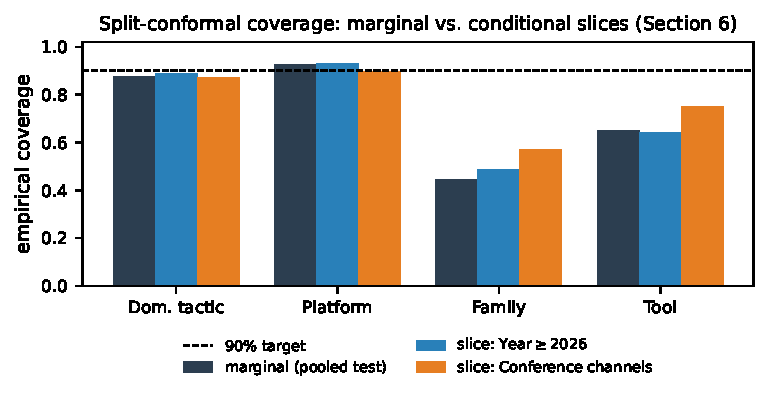
\includegraphics[width=0.85\textwidth]{figures/fig_conformal_coverage.pdf}
  \caption{Empirical conformal coverage, marginal vs.\ the two
    conditional-coverage stress-test slices, against the 90\% target
    (\Cref{tab:conformal}).}
  \label{fig:conformal}
\end{figure}

\section{Out-of-Distribution Detection}
\label{sec:ood}
Unlike Sections~\ref{sec:baselines}--\ref{sec:conformal}, this section's
results are not subject to the weak-label scope note in
Section~\ref{sec:gold-scope}: OOD detection asks whether a model's own
confidence or embedding-space behavior differs between in-distribution
and out-of-distribution input, which is answerable without knowing
whether either input's \emph{label} is correct.

\subsection{Setups and methods}
\label{sec:ood-setups}
Four setups, each with a known-by-construction in-distribution
(ID)/out-of-distribution (OOD) split, drawn from real structure in the
corpus rather than synthetic corruption:

\begin{enumerate}
\item \textbf{Temporal emergence.} ID: pre-2024 videos. OOD: post-2024
  videos mentioning a family whose first appearance in this corpus is
  2024 or later -- verified directly against per-family first-occurrence
  year rather than assumed (Maze, Medusa, Black Basta, INC: 2024;
  Cactus: 2025), at \Cref{alg:ood-verify}'s assertion step.
\item \textbf{Channel-type shift.} ID: Vendor + DFIR channels. OOD:
  Conference + Independent channels.
\item \textbf{Leave-rare-family-out.} ID: videos never mentioning
  ``Cl0p'' (11 occurrences total -- long-tailed, unlike Conti/LockBit/
  Qilin/Akira, each with 19+). OOD: the 11 Cl0p-mentioning videos.
\item \textbf{External corpus.} ID: RansKnow transcripts. OOD: 20
  Newsgroups (\texttt{rec.sport.baseball} + \texttt{sci.space}), included
  as a sanity check that the methods below can detect an obviously
  unrelated domain before trusting them on setups 1--3.
\end{enumerate}

Four detection methods, computed from a shared \texttt{dominant\_tactic}
classifier (structured features, LightGBM -- \Cref{tab:results}'s
strongest non-circular result, and a natural multiclass fit for the
softmax-family methods below), refit fresh on each setup's ID-only
training pool so that no OOD signal leaks into fitting:
\begin{align}
  s_{\mathrm{MSP}}(x) &= 1 - \max_c \hat p(c\mid x)
    \label{eq:msp}\\
  s_{\mathrm{energy}}(x) &= -\log\sum_c \exp\bigl(f_c(x)\bigr)
    \label{eq:energy}\\
  s_{\mathrm{maha}}(x) &= \min_c \bigl(\phi(x)-\mu_c\bigr)^{\!\top} \Sigma^{-1} \bigl(\phi(x)-\mu_c\bigr)
    \label{eq:maha}\\
  s_{\mathrm{conf}}(x) &= 1 - \hat p\bigl(\hat c(x) \mid x\bigr) \qquad\text{(\Cref{eq:lac} at the predicted class)}
    \label{eq:conf-ood}
\end{align}
\Cref{eq:msp} is Hendrycks and Gimpel's max-softmax-probability baseline
\citep{hendrycks2017baseline}. \Cref{eq:energy} is the energy score
\citep{liu2020energy}, computed from LightGBM's raw pre-softmax margins
$f_c(x)$ (\emph{not} from $\hat p(c\mid x)$: probabilities already sum to
$1$, which makes \Cref{eq:energy} degenerate to a constant if computed
from them directly -- a real pitfall caught while implementing this
section, not a hypothetical one). \Cref{eq:maha} is the class-conditional
Gaussian Mahalanobis distance of \citet{lee2018simple}, with $\phi(x)$ the
384-dim mean-pooled sentence embedding (\Cref{sec:baselines}'s footnote)
and $\mu_c,\Sigma$ the ID-train class-conditional means and pooled
covariance, using the classifier's own \emph{predicted} classes to form
groups (consistent with \Cref{sec:gold-scope}: no independently verified
labels exist to group by instead). \Cref{eq:conf-ood} reuses
\Cref{sec:conformal}'s LAC score, evaluated at the predicted rather than
true class for OOD flagging -- this is deliberately, not accidentally,
the same quantity as \Cref{eq:msp}; the two are reported separately for
comparability with \Cref{eq:qhat}'s calibrated threshold (does a point's
own score exceed the 90\%-target $\hat q$), which is the operationally
distinct number.

\begin{algorithm}[htbp]
\caption{OOD setup evaluation}
\label{alg:ood-verify}
\begin{algorithmic}[1]
\Require corpus $\mathcal{D}$, ID/OOD partition rule for the setup
\State \textbf{assert} every claimed-emerging family's first-occurrence year matches the setup's stated cutoff \Comment{caught a factual error at this step -- see note below}
\State split ID pool into $\mathcal{D}_{\mathrm{train}}$ (75\%) / $\mathcal{D}_{\mathrm{test}}^{\mathrm{ID}}$ (25\%)
\State fit \texttt{dominant\_tactic}/structured/LightGBM on $\mathcal{D}_{\mathrm{train}}$
\State score $\mathcal{D}_{\mathrm{test}}^{\mathrm{ID}}$ and $\mathcal{D}_{\mathrm{OOD}}$ under \Cref{eq:msp,eq:energy,eq:maha,eq:conf-ood}
\State report AUROC(ID vs.\ OOD) per method, plus the conformal exceedance-rate contrast
\end{algorithmic}
\end{algorithm}

The assertion in \Cref{alg:ood-verify} is not decorative: the temporal-
emergence setup's family list was originally drafted from memory as
``Qilin, DragonForce, Black Basta,'' before checking actual
first-occurrence years against the corpus. Qilin's first real occurrence
is 2019, not post-2023, and DragonForce does not appear in this corpus at
all -- both would have silently produced a meaningless setup (there is no
real ID/OOD separation if the ``emerging'' families already appear
throughout the ID training period). The corrected list (Maze, Medusa,
Black Basta, INC, Cactus) is the one actually used in \Cref{tab:ood} and
is verified by \Cref{alg:ood-verify} on every run, not just checked once
by hand.

\subsection{Results}
\label{sec:ood-results}
\begin{table}[htbp]
\centering
\caption{OOD-detection AUROC by setup and method (\Cref{eq:msp,eq:energy,eq:maha,eq:conf-ood}).
  $n_{\mathrm{ID}}$/$n_{\mathrm{OOD}}$ are ID-test/OOD sample counts.
  Mahalanobis is unavailable for \texttt{external\_corpus} (20
  Newsgroups has no entry in the RansKnow-only embedding cache).}
\label{tab:ood}
\begin{tabular}{lrrrrrr}
\toprule
Setup & $n_{\mathrm{ID}}$ & $n_{\mathrm{OOD}}$ & MSP & Energy & Mahalanobis & Conformal \\
\midrule
Temporal emergence     &  55 &   31 & 0.561 & 0.360 & 0.223 & 0.533 \\
Channel-type shift       & 156 &  353 & 0.477 & 0.487 & 0.666 & 0.487 \\
Leave-rare-family-out    & 256 &   11 & 0.377 & 0.350 & 0.145 & 0.376 \\
External corpus (sanity) & 259 & 1190 & 0.625 & 0.476 & --    & 0.631 \\
\bottomrule
\end{tabular}
\end{table}

\Cref{fig:ood-radar} plots \Cref{tab:ood}. The honest reading is a mixed
and mostly negative one, which is itself the finding worth reporting
rather than a result to explain away. Three observations:

\textbf{The confidence-based methods (MSP, energy, conformal) hover near
chance (0.5) on every setup, including the sanity check.} Diagnosing
\emph{why} on \texttt{external\_corpus} is informative: 99.6\% of 20
Newsgroups documents are classified \texttt{None} (no dominant tactic
detected) by the shared classifier, and with \emph{higher} average
confidence than the real in-distribution test set (mean $\hat
p_{\max}$: 0.921 OOD vs.\ 0.895 ID). A near-empty, off-topic TF-IDF
vector and a genuinely tactic-free ransomware transcript both produce
the same signature -- confidently ``no tactics detected'' -- so a
classifier whose decision function is fundamentally an argmax over
small keyword-mention counts has no way to distinguish ``nothing here''
from ``wrong domain entirely.'' This is a known blind spot of
softmax/probability-based OOD detection in general
\citep{hendrycks2017baseline}, reproduced concretely here rather than
assumed from the literature.

\textbf{Mahalanobis distance on real sentence embeddings is the one
method that separates classes at all, and only partially.} It reaches
$0.666$ on channel-type shift -- Conference/Independent channels differ
enough in embedding space (production style, framing, audience) to be
mildly detectable -- but performs \emph{worse} than chance on temporal
emergence (0.223) and leave-rare-family-out (0.145). Both of those
setups' OOD population describes the same underlying phenomenon
(ransomware incidents, attacker tradecraft) as the ID population, just
naming a different or newer group -- exactly the case where sentence
embeddings, which encode semantic content rather than proper nouns,
would \emph{not} be expected to separate the two populations well. The
small OOD sample sizes in these two setups ($n{=}31$, $n{=}11$) also mean
each AUROC estimate carries substantial variance on its own; with
$n_{\mathrm{OOD}}{=}11$, a single re-ordered pair moves the estimate by
roughly $1/11$.

\textbf{The conformal exceedance-rate contrast (\Cref{eq:qhat}'s $\hat
q$) is uninformative in this corpus specifically.} In every setup, the
calibrated threshold $\hat q$ lands so close to the maximum possible
score ($\hat q \geq 0.99$ in three of four setups) that essentially no
point, ID or OOD, exceeds it -- a consequence of the classifier being
very confidently correct on the bulk of its small ($n{\approx}115$)
calibration split, which pushes the $90$th-percentile score to an
extreme value. \Cref{eq:conf-ood}'s AUROC column is the more informative
number from this method here; the exceedance-rate contrast is reported
in the released JSON (\texttt{outputs/phase4\_ood.json}) for
completeness but is not a useful discriminator at this sample size.

\begin{figure}[htbp]
  \centering
  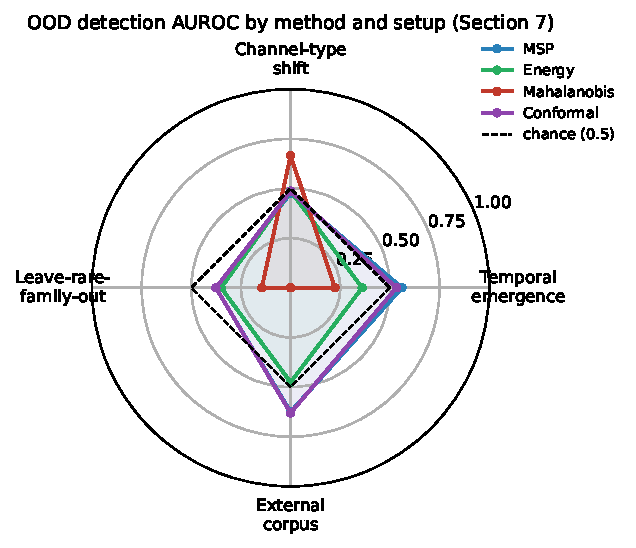
\includegraphics[width=0.6\textwidth]{figures/fig_ood_radar.pdf}
  \caption{OOD-detection AUROC by method (color) and setup (axis),
    against the chance line at 0.5 (\Cref{tab:ood}). Mahalanobis is the
    only method to clear chance by a wide margin, and only on one of
    four setups.}
  \label{fig:ood-radar}
\end{figure}

Taken together, \Cref{sec:ood-results} does not support a general claim
that this pipeline's models reliably detect distributional shift; it
supports a narrower, still useful one: OOD detection here is hard,
softmax-confidence-based methods have an identifiable and reproducible
blind spot on this specific classifier (the ``no signal'' vs.\
``wrong domain'' confusion above), and embedding-distance methods help
only when the shift is stylistic rather than topical. Unlike
\Cref{sec:baselines,sec:uncertainty,sec:conformal}, none of this depends
on whether $y^{\mathrm{KA}}$ is correct (\Cref{sec:gold-scope}) -- it is
a direct, if modest, empirical finding about model behavior.

\section{Interpretability and Perturbation Robustness}
\label{sec:interpretability}
Unlike Sections~\ref{sec:baselines}--\ref{sec:conformal}, this section
asks questions about model \emph{behavior} -- does it exploit shortcuts,
what does it rely on, how much do its predictions move under
semantically-irrelevant edits -- none of which require independent
ground truth to answer, so Section~\ref{sec:gold-scope}'s scope note
does not apply here.

\subsection{Confound checks}
\label{sec:confounds}
\textbf{Length.} Transcript word count correlates moderately with
\texttt{Tactic\_Total\_Mentions} (Pearson $r=0.409$) and weakly with
\texttt{Family\_Count} ($r=0.131$), but not at all with
\texttt{Tool\_Total\_Mentions} ($r=0.043$, not significant) -- the
confound is not uniform across signal types. Because it is mathematically
guaranteed that dividing every tactic's count for one video by that
video's own word count cannot change which tactic has the highest count
(argmax is scale-invariant per row), the confound cannot affect how the
\texttt{Dominant\_Tactic} label itself was derived; the question that
matters is whether it inflates \texttt{dominant\_tactic}'s strongest
result (structured features, \Cref{tab:results}). Re-scoring with
length-normalized (mentions per 1{,}000 words) instead of raw-count
features gives 0.753 macro-F1 against the raw-count model's 0.764 -- a
1.1-point difference, not a length-exploitation artifact.

\textbf{Channel identity.} 486 of 1{,}034 transcripts (47\%) contain at
least one literal mention of their own channel's name. Masking those
mentions and re-scoring TF-IDF LogReg under both CV protocols leaves the
\texttt{channel\_grouped}-vs-\texttt{stratified\_random} gap unchanged
for \texttt{family} (0.028 raw $\to$ 0.031 masked) and for
\texttt{dominant\_tactic} (0.020 raw $\to$ 0.029 masked). Whatever a
model exploits when a channel is not held out, it is not the channel
literally naming itself -- the leakage this split protocol exists to
catch is stylistic or topical, not addressable by name-masking.

\subsection{Counterfactual explanations}
\label{sec:counterfactual}
Motivated directly by Finding A: does a classifier trained on the
\emph{fixed} labels still show the regex's original word-collision
fragility? A TF-IDF+LogReg model was trained on today's corrected
\texttt{Family} labels and evaluated on the 275 videos Section~\ref{sec:finding-a}
confirmed as false positives under the pre-fix regex (videos where
``\texttt{play}'' appears without ransomware context). The trained model
assigns essentially zero probability to \texttt{Play} on all 275
(maximum $P=0.013$) -- it did not inherit the bare-word-collision bug.

The complementary question -- what drives the model's actual positive
\texttt{Play} predictions -- was then asked with a greedy word-\emph{type}
removal counterfactual search (remove the vocabulary word whose removal
most reduces $P(\text{Play})$, repeat until the prediction flips or a
budget is exhausted) on the 8 highest-confidence true positives.
\texttt{play} appears in 5 of 8 removal sets and is consistently one of
the highest-impact single removals when present, but \textbf{0 of 8
cases flip on removing ``play'' alone} -- every flip required 4--10
additional removals, most of them generic (function words, not
ransomware-specific vocabulary). The model reduced, but did not
eliminate, reliance on the single ambiguous trigger word, and the words
it combines that reliance with are not obviously a clean, interpretable
``ransomware vocabulary'' set -- worth flagging as its own finding about
decision-boundary diffuseness, independent of the word-collision
question it was designed to answer.

\subsection{Perturbation robustness}
\label{sec:perturbation}
Untargeted counterpart to the counterfactual search above: two
perturbation types, measuring flip rate (does the top prediction change)
and mean absolute probability drift on freshly-fit TF-IDF+LogReg models.
\emph{Simulated ASR noise} (compound proper nouns split apart, e.g.
\texttt{WannaCry}$\to$``wanna cry,'' \texttt{Mimikatz}$\to$``mimi cats,''
plus 8\% random token deletion) was applied to the 74 official-caption
videos specifically -- the ``clean'' subset, simulating what those
transcripts would look like if they had gone through the ASR cascade
that produced the other 92.7\% of the corpus (Finding B). \emph{Synonym
substitution} (common non-jargon words swapped for synonyms) was applied
to a 150-video sample.

\texttt{dominant\_tactic}, \texttt{platform}, and \texttt{relevance} are
essentially unmoved by either perturbation (0.0--0.7\% flip rate, mean
drift $<0.01$ in every case). \texttt{family} flips 20--26\% of the time
under both perturbations despite a much smaller mean drift ($\sim$0.002)
than any other task -- not a new problem, but the same weak-model issue
from \Cref{tab:results} (\texttt{family}'s best macro-F1 is 0.129)
surfacing differently: closely-bunched, low-confidence probabilities
mean a negligible nudge is enough to change which barely-ahead class
wins. On the framing of ``adversarial'' robustness for this dataset: no
real adversary submits transcripts to evade this classifier in
production, so a full gradient-based adversarial-attack framework would
be disproportionate to what this paper needs; the actual risk surface is
ASR transcription noise and channel-style variation, which is what this
sweep directly measures. Combined with Section~\ref{sec:ood}'s
temporal-emergence and leave-rare-family-out setups, these results are
the paper's answer to how the system handles evolving, novel, and
adversarial-adjacent input -- not three separate open questions.

\section{Limitations and Ethics}
\label{sec:limitations}

\todo[inline]{Expand into full prose; bullets below are the content, not
    the final form. The first bullet is the paper's central limitation and
    should probably open this section as prose, not sit inside a list with
    four other items of noticeably smaller consequence.}
\begin{itemize}
  \item \textbf{No independent ground truth.} This is the paper's central
    limitation, not one bullet among several, and is why it is stated
    repeatedly rather than once: this project does not include a
    human-annotated evaluation set independent of the Knowledge Agent
    pipeline (Section~\ref{sec:gold-scope}). External annotator recruitment
    required institutional ethics approval not available to this project;
    a single-investigator annotation pass was considered and rejected as
    still too close to the system under evaluation to count as independent
    evidence. Every result in Sections~\ref{sec:baselines}--\ref{sec:conformal}
    is consequently agreement with an audited but demonstrably imperfect
    extraction pipeline (Finding A), not verified accuracy -- Section~\ref{sec:ood}'s
    OOD results and Section~\ref{sec:interpretability}'s behavioral
    diagnostics are the exceptions, since neither depends on label
    correctness. Recruiting independent annotators, whether through formal
    ethics approval or an unpaid collaborator arrangement that falls
    outside whatever definition of human-subjects research applies at the
    author's institution, is the single highest-value extension of this
    work -- more valuable than any additional modeling in
    Sections~\ref{sec:baselines}--\ref{sec:conformal} would be, since none
    of that modeling can currently be checked against anything but itself.
  \item \textbf{Sampling bias.} The corpus is conditioned on which
    channels operators chose to run, which videos they chose to title and
    describe in keyword-matchable ways, and YouTube's own recommendation
    and search surfacing -- not a random or exhaustive sample of
    ransomware-relevant discourse.
  \item \textbf{ASR noise.} 92.7\% of transcripts are machine-transcribed,
    mostly by \texttt{whisper\_base}. Section~\ref{sec:perturbation}'s
    simulated-ASR-noise sweep bounds how much this moves predictions;
    Finding B's word-error-rate-on-jargon question (comparing ASR output
    against source audio directly, rather than a simulation of ASR-style
    errors) remains open.
  \item \textbf{Weak-label ceiling.} Every quantitative result in
    Sections~\ref{sec:baselines}--\ref{sec:conformal} is bounded by the
    Knowledge Agent's own precision/recall, which Finding A shows is not
    perfect even after the disambiguation fix, and which
    Section~\ref{sec:counterfactual} shows partially propagated into at
    least one trained model.
  \item \textbf{Dual use.} This is a corpus of ransomware tactics, tools,
    and case studies extracted from public educational content. \todo{Add
      a considered dual-use statement -- the underlying source material is
      already public (YouTube videos aimed at defenders), but structuring
      it may lower the effort to extract offense-relevant patterns; discuss
      how this compares to existing public MITRE ATT\&CK mappings and
      threat-intel reporting, which already aggregate similar information.}
\end{itemize}

\section{Conclusion}
\label{sec:conclusion}
\todo[inline]{Write last. Should state the label-quality audit
    methodology and code (Section~\ref{sec:audit}, Section~\ref{sec:interpretability})
    as a second contribution alongside the transcripts themselves -- other
    weak-label security-NLP datasets built the same way (keyword/regex
    extraction over scraped text) can reuse the audit methodology even
    without reusing the corpus. Should also state candidly that the most
    valuable open follow-up to this specific paper is independent
    human-annotated verification (Section~\ref{sec:limitations}), not
    further modeling -- and should say why explicitly rather than
    trailing off: every result this paper reports beyond
    Section~\ref{sec:ood} would change in \emph{meaning}, not just in
    number, the day that verification exists.}

\begin{ack}
\todo[inline]{Funding and competing-interest disclosure required here
    per NeurIPS 2026 policy (\url{https://neurips.cc/Conferences/2026/PaperInformation/FundingDisclosure}).
    This section is auto-hidden in the anonymized submission by the
    \texttt{ack} environment (see \texttt{neurips\_2026.sty}) -- do not
    remove it or move this content elsewhere expecting the same
    behavior.}
\end{ack}

\bibliographystyle{plainnat}
\bibliography{references}

\appendix
\section{Keyword List}
\label{app:keywords}
\todo[inline]{Insert the full \texttt{KEYWORDS} list from
    \texttt{Scripts/fetch\_transcripts.py} verbatim.}

\newpage
\input{checklist.tex}

\end{document}
